% -*- TeX:de -*-
\NeedsTeXFormat{LaTeX2e}
\documentclass[12pt,a4paper,titlepage]{article}

\usepackage[german]{babel} % german text
\usepackage[DIV12]{typearea} % size of printable area
\usepackage[T1]{fontenc} % font encoding
\usepackage[latin1]{inputenc} % most likely on Windows
%\usepackage[utf8]{inputenc} % probably on Linux

\usepackage{graphicx} % to include images
%\usepackage{subfigure} % for creating subfigures
\usepackage{amsmath} % a bunch of symbols
\usepackage{amssymb} % even more symbols
\usepackage{booktabs} % pretty tables

% a floating environment for circuits
\usepackage{float}
\newfloat{circuit}{tbph}{circuits}
\floatname{circuit}{Schaltplan}
\restylefloat*{circuit}

% a floating environment for diagrams
\usepackage{float}
\newfloat{diagram}{tbph}{diagrams}
\floatname{diagram}{Diagramm}
\restylefloat*{diagram}

\renewcommand{\familydefault}{\sfdefault} % use sans-serif font as default

\selectlanguage{german} % use german
\sloppy % friendly typesetting
\setlength\parindent{0pt} 

\begin{document}

% Titelblatt
%%%%%%%%%%%%%%%%%%%%%%%%%%%%%%%%%
% create title page
%%%%%%%%%%%%%%%%%%%%%%%%%%%%%%%%

\begin{titlepage}

\begin{figure}[h!]
	\centering
  
\includegraphics[width=5cm]{JKULogokurzWappenlinks_ger.jpg}
\end{figure}

\begin{center}
\vspace*{1.3cm}
{\Large Spezielle Kapitel der Informatik:\\Music Information Retrieval\\KV SS2009\\}
\vspace{4cm}
{ Protokoll der "Ubungsaufgabe:\\}{\huge Informationsextraktion mit LastFM \\ im Vergleich mit Google\\}
\vspace{4 cm}

% fill in group number and date of lab here
% CHANGE ME!
{\Large Datum der Pr"asentation: 24. Juni 2009}
\vspace{0.5cm}


% fill in IDs and names here
% CHANGE ME!
\begin{table}[h!]
\centering
\begin{tabular}{|p{3.5cm}|p{3.5cm}|p{6.5cm}|}
\hline \textbf{Matr. Nr.} & \textbf{Kennzahl} & \textbf{Name} \\
\hline
& & Jakob Doppler\\
\hline
& & Doris Zachhuber\\
\hline
0856711 & 086 & Matthias Husinsky\\
\hline
\end{tabular}
\end{table}

\end{center}

\end{titlepage}
\setcounter{page}{2}

%%%%%%%%%%%%%%%%%%%%%%%%%%%%%%%%
% start of actual document
%%%%%%%%%%%%%%%%%%%%%%%%%%%%%%%%

\newpage
\tableofcontents

% Ueberblick
\newpage
\section{Einleitung}

\subsection{Aufgabenstellung}
Im Zuge der LV \textit{Music Information Retrieval} war der �bungsteil im Rahmen einer Gruppenarbeit zu erledigen. Kurz gefasst bestand die Aufgabe darin, ein Music Information System - in unserem Fall LastFM auf dessen Features zu untersuchen und unter dessen Zuhilfenahme Informationskategorien zu extrahieren und darauf aufbauend Features und �hnlichkeitsma�e zu berechnen.

\subsection{Zielsetzungen}
LastFM ist ein, im Vergleich zu anderen MIS Services, relativ ausgereifter Dienst mit einer gro�en Useranzahl, weshalb er auch gerne f�r MIR-Tasks verwendet wird.

Wir setzten uns zum Ziel diesesn Dienst zur Datenaggregation zu verwenden, um die gewonnen Infos in weiterer Folge zur Feature- und �hnlichkeitsberechnung zu verwenden. Extrahiert wurden zur weiteren Verwendung die Bands hinzugef�gten und gewichteten Tags sowie die Releasedaten der Alben der K�nstler. Mithilfe letzerer wurden ein neu erfundenes Feature der \textit{Wirkzeit} berechnet und untersucht. Die Tags wurden zur �hnlichkeitsberechnung von K�nstlern untereinander verwendet.

Zus�tzlich wurden aufgrund der einfachen Zug�nglichkeit der Daten mittels einer API noch allgemein im Web verf�gbare Daten (mittels Google-Recherche) akkumuliert, analysiert und anschlie�end mit den Daten aus aus LastFM verglichen.

Eine grobe Visualisierung der gewonnen Erkenntnisse sollte die Erschlie�barkeit f�r den Nutzer unterst�tzen. 

Zu guter Letzt wurden noch ein paar Experimente zur Genre-Klassifizierung von K�nstlern aus den gewonnenen Daten vorgenommen.

% Ueberblick
\newpage
\section{LastFM}
\subsection{Hintergrund}
\textit{LastFM} ist heute ein personalisiertes Online-Radio - abspielbar mit einer eigenen, propri"ateren Software. Dieses erm"ogicht es den Usern, einen eigenen, auf ihren Geschmack zugeschnittenen Musikstream abzuspielen. Angegeben kann der momentan gew"unschte Musikstil via Tags, entweder auf einen K"unstler bezogen, oder auf einen Musikstil bzw. Genre. Ebenso ist es m"oglich via Plug-Ins das Abspielverhalten von andere Audio-Playern zu beobachten um die Erstellung des Nutzerprofils zu unterst"utzen.
Weiters ist \textit{LastFM} auch ein gro"ses soziales Netzwerk, dass vor allem auf das zusammenbringen von Menschen mit "ahnlichem Musikgeschmack ausgelegt ist. Die User der Community tragen zur Klassifikation des Musikbestandes durch tagging, Wiki-Betr"age und einfach ihr H"orverhalten bei. Mehr dazu in Abschnitt \ref{features_lastfm}.

\subsection{Geschichtlicher "Uberblick}
\textit{LastFM} wurde in den sp"aten 90er Jahren als Online-Musiklabel gegr"undet und bot als Feature die M"oglichkeit, sich durch die Art der konsumierten Musikst"ucke ein Profil "uber seinen Musikgeschmack zu erstellen zu erstellen. Die Firma \textit{Audioscrobbler}, hervorgegangen aus einem Informatikprojekt, hatte sehr "ahnliche Ideen, worauf hin beide Unternehmen sehr eng zusammenarbeiteten, bis sie schlie"slich im Jahr 2005 fusionierten und unter dem Namen \textit{LastFM} die Funktionen von beiden Technologien zur Verf"ugung stellen.
2007 wurde \textit{LastFM} um den Preis von 280 Millionen Dollar an das US-amerikanische Medienunternehmen CBS verkauft. Diese "Ubernahme geh"ort damit zu den gr"o"sten dotcom Aquisitionen bisher. 
Seit April 2009 ist die Benutzung des Radiodienstes nur mehr in den USA, Gro"sbritannien und Deutschland kostenlos m"oglich. In anderen L"andern muss ein entgelt von 3 Euro f"ur die monatliche Nutzung erbracht werden.





% System Architecture
\newpage
\section{Systemarchitektur}

Bei der Implementierungsarbeit zum Projekt wurde auf eine schlanke, modular gekapselte und erweiterbare Systemarchitektur zur Erfassung, Verarbeitung und Analyse der Daten aus verschiedenen Musikinformationsquellen geachtet. Aufgrund der einfach zu handhabenden prototypischen Entwicklung und gute Unterst�tzung durch Open Source Bibliotheken von Drittherstellern wurde Java innerhalb Eclipse IDE als Zielsprache gew�hlt. 


\subsection{MIR Framework}

Der Hauptanteil der Entwicklung fokusiert sich auf die Datenerfassung und Aufbereitung verschiedenster deskriptiver und numerischer Eigenschaften aus unterschiedlichsten Datenquellen zu einer K�nstler Entit�t \texttt{MirArtist}. Abb.~\ref{fig:systemarchitecture} zeigt die Grundz�ge der Systemarchitektur, die in f�nf Ebenen gegliedert ist. Neben der Datenerfassung, Informationsextraktion und �hnlichkeitsberechung wurde auch Wert auf die visuelle Aufbereitung der Ergebnisse in Form von Charts, Netzwerkgraphen und Clustern gelegt. Drei heterogene \textbf{Datenquellen} wurden zur Erfassung von k�nstlerbezogenen Features herangezogen:
\begin{figure}[ht]
	\centering
	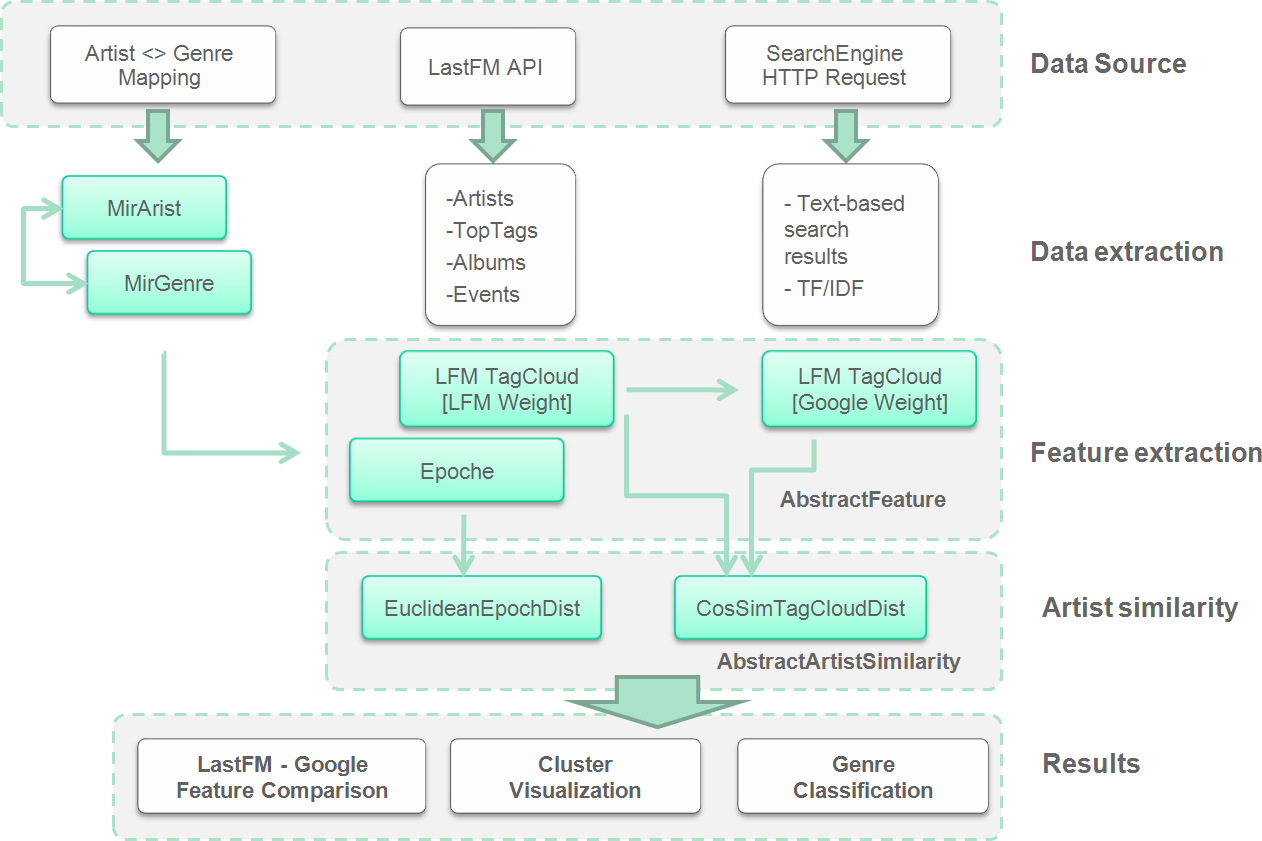
\includegraphics[width=0.8\textwidth]{images/systemarchitecture.png} % \textwidth
	\caption{System Architektur des im Rahmen des Projekts entwickelten MIR Frameworks}
	\label{fig:systemarchitecture}
\end{figure} 


\begin{itemize}
	\item \textbf{Artist-Genre Mapping:} Das Textfile-basierte Mapping von 224 K�nstlern (je 11 in 14 Genres) war Teil der �bungsbeschreibung.
	\item \textbf{LastFM API:} Die API zu dem Musikportal LastFM war die Hauptquelle zur Erfassung vieler k�nstlerbezogener Daten wie etwa TopTags, Album Release Dates, Auftrittsorte (Events und Venues). F�r die SOAP-basierte Schnittstelle stand eine Java-Bibliothek zur Verf�gung. Diese wurde modifiziert um neben den Top Tags auch die Tag-Gewichte f�r akkurater �hnlichkeitsberechungen erfassen zu k�nnen.
	\item \textbf{Search Engine Queries:} Um einen Vergleich zwischen den �hnlichkeiten der Community-basierten LastFM Platform und einer nicht Benutzergetrieben Datenqueller herstellen zu k�nnen, wurde ein dem CoMIRVA Framework angelehnter \texttt{UrlRetriever} f�r Suchmaschinenabfragen implementiert, der auf Basis der ersten $N$ Linkresultate in Google ein UrlDownloader zum Download der Pages anregt.
\end{itemize}

Auf Ebene der \textbf{Featureextraktion} wurde eine Basisklasse \texttt{Feature} eingef�hrt, die die Heterogenit�t der k�nstlerbezogenen Eigenschaften wie Genrezugeh�rigkeit, listenbasierter Tag-Wolken und Schaffensperiode aus den Grunddaten extrahiert. Dese Features k�nnen nicht direkt instanziert werden, sondern werden durch eine \texttt{FeatureFactory}, die den Zugriff zum Datenlayer kapselt, generiert. Jedes abstrakte Feature kann anschlie�end unter einem gemeinsamen Interface beim zugeh�rigen Artist registiert werden. 

F�r die \textbf{�hnlichkeitsberechung }wurde ebenfalls eine \texttt{AbstractSimilarityMeasure} Basisklasse definiert, die die Ableitung von konkreten Klassen zur Berechung von symmetrischen �hnlichkeitsmatrizen zwischen $NxN$ K�nstlern erlaubt. Jedes �hnlichkeitsma� wei� �ber den internen Aufbau eines konkreten Features Bescheid und kann auf dieses unter Zuhilfenahme einer eindeutigen FeatureID darauf zugreifen falls das Feature zuvor berechnet und registriert wurde. Abb.\ref{fig:flowchart} zeigt das Flussdiagramm einer modularen Featureaggregation innerhalb eines einzelnen K�nstlern. Sofern f�r jedes Feature oder eine Sammmlung an Features ein entsprechendes SimilarityMeasure implementiert wurde kann ein numerische �hnlichkeitsmatrix als normiertes \textbf{Resultat} f�r die textbasierte Interpretation, eine Visualisierung aber auch einen Genre-Klassifikationversuch herangezogen werden. 

\begin{figure}[ht]
	\centering
	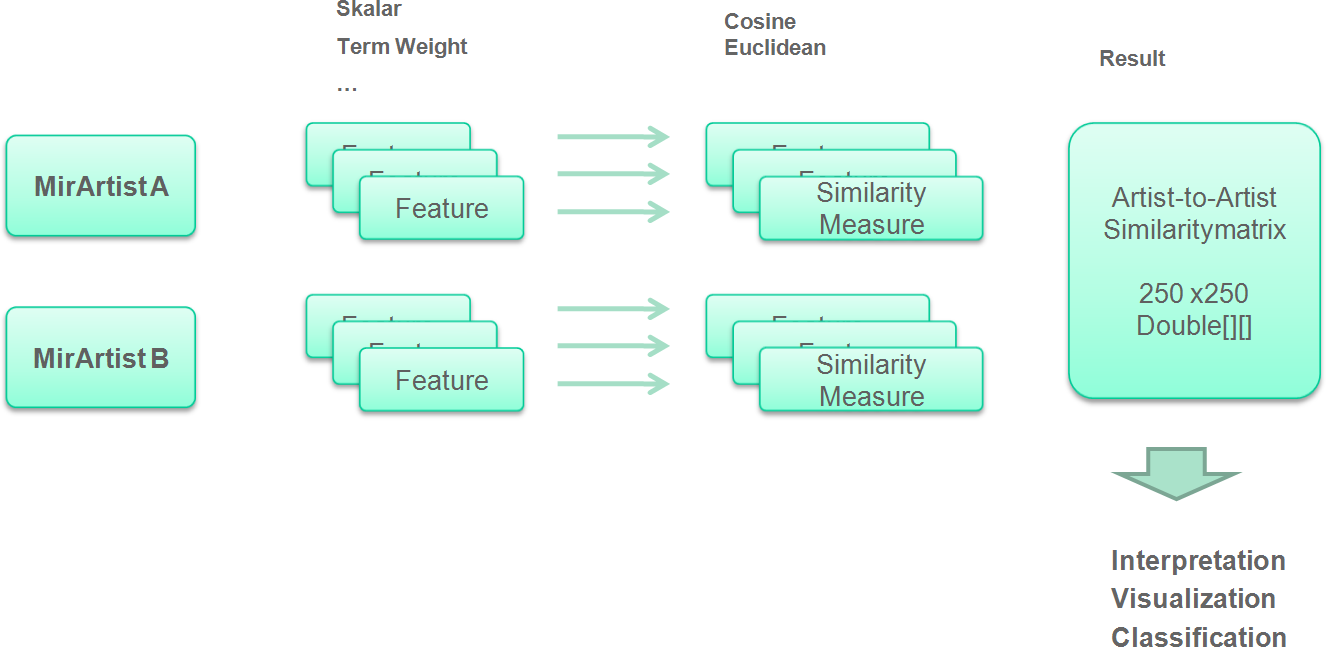
\includegraphics[width=0.7\textwidth]{images/flowchart.png} % \textwidth
	\caption{Informationsextraktion - \texttt{MirArtist} vereinheitlichte Datenaggregation}
	\label{fig:flowchart}
\end{figure} 


\subsection{Metriken und Tools}

Im Zuge des Projekts wurden unter Verwendung einiger stark modifizierter Fremdklassen �ber 4000 LoC in 60 Klassen (11 Packages) entwickelt. Abb.~\ref{fig:mainclasses} zeigt in einem Abh�ngigkeitsgrafen die Hauptklassen rund um die \texttt{MirArtist}-Entit�t. Die flexible Architektur und gute Kapselung der Teilaufgaben erm�glichte ein rasches Prototyping und gro�e Wiederverwendbarkeit vor allem des Feature Registrierungsmechanismusses und der abtrakten Klassen zur �hnlichkeitsberechung. Die Entwicklungzeit jedes weiteren Features konnte damit drastisch gesenkt werden und erm�glichte eine umfangeiche Analyse zur Dateninterpretation, Vergleichsberechung und zu anschlie�enden Visualisierungs- und Klassifikationsversuchen.

\begin{figure}[ht]
	\centering
	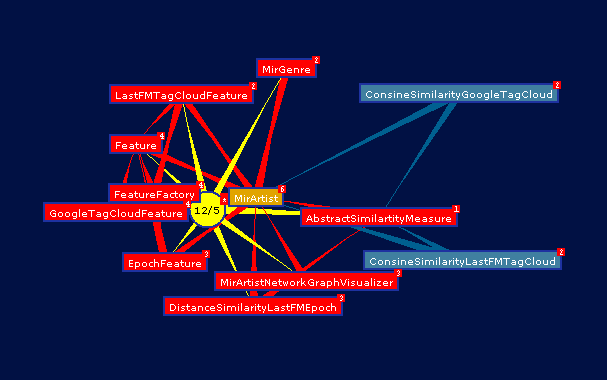
\includegraphics[width=0.6\textwidth]{images/classes.png} % \textwidth
	\caption{Visualisierter Abh�ngigkeitsgraph der Hauptklassen rund um \texttt{MirArtist}.}
	\label{fig:mainclasses}
\end{figure} 





% Angewandte Methoden
\newpage
\section{Auswertung der Daten}


\subsection{Datenquellen}
\subsubsection{Textbasiertes Genre-Artist-Mapping}
Verwendet f�r...

\subsubsection{LastFM}
Verwendet f�r Albeninfos f�r Berechnung der Wirkungszeit und f�r TagClouds, auch als Ground-Truth f�r die Klassifizierung, sowie f�r die Berechnung der aktivsten Wirkungszeit eines K�nstlers basierend auf den Releasedates seiner Alben. Dazu braucht man einen aktiven Account und api-key,.... (JAKOB)


\subsubsection{Google}
TagClouds durch Termfrequency

\subsection{Feature Extraction}
\subsubsection{Albumbasierte Wirkungszeit} \label{feature_wirkungszeit}
F�r die aktivste Wirkungszeit eines K�nstlers wurde ein Feature (skalarer Datenwert) berechnet, das mit Hilfe der LastFM-API ermittelt wurde. Die Wirkungszeit eines K�nstlers kann (muss aber nicht) repr�sentativ f�r eine bestimmte Epoche sein. Der letzte Fall trifft vor allem bei K�nstlern zu, die �ber mehrere Jahrzehnte hinweg aktiv sind, da sie nicht zwingend einer herk�mmlichen Epoche wie den 70ern oder 80ern, etc.\ zugeordnet werden k�nnen. 

Die aktivste Wirkungszeit wurde anhand der Anzahl und des Erscheinungsjahres der ver�ffentlichten Alben eines K�nstlers berechnet. Dazu wurden s�mtliche Alben inkl. deren Releasedates mit Hilfe der LastFM-API extrahiert. Die API stellt dazu die Funktion \texttt{artist.getTopAlbums} zur Verf�gung. Von den zur�ckgegebenen Alben k�nnen in der Folge mit der Funktion \texttt{album.getInfo} n�here Infos, u.a. das ReleaseDate des Albums, abgefragt werden.

F�r die Berechnung des Features wurden s�mtliche Releasedates addiert und ihr \textit{Mittelwert} gebildet. Es soll das mittlere Jahr der gesamten (bisherigen) Wirkungszeit repr�sentieren. 

\subsubsection{TagClouds}


\subsection{�hnlichkeitsmessungen}
\subsubsection{Differenz von skalaren Werten}
Das in Kap.\ \ref{feature_wirkungszeit} berechnete Feature wurde f�r die Berechnung des �hnlichkeitsma�es verwendet. Dieses soll darstellen, welche K�nstler zur selben Zeit am aktivsten (hinsichtlicher der produzierten Alben) waren. Optimalerweise l�sst sich daraus auch eine gewisse Genre�hnlichkeit der K�nstler feststellen, da gewisse Genres, z.B. Electronic, Punk, etc. sehr typisch f�r gewisse Zeitepochen der Geschichte sind. F�r Rock, Pop oder Heavy Metall trifft das kaum oder gar nicht zu.

Die H�he der �hnlichkeit wurde aus der Distanz zwischen den skalaren Featurewerten zweier K�nstler berechnet. Je n�her sich die Features selbst waren (�hnliche Jahreszahlen), desto geringer ist die Differenz. Folglich musste diese Distanz (nach erfolgter Normalisierung anhand der Featurewerte) invertiert werden, damit h�here Werte ein h�heres Ma� an �hnlichkeit ausdr�cken. Letztendlich bewegt sich diese zwischen den Werten 0.0 (keine �hnlichkeit) und 1.0 (idente aktivste Wirkungszeit). 

\subsubsection{Cosinus-Similarity}
Ein Ma"s zur Bestimmung der "Ahnlichkeit der K"unstler in der LastFM Datenbank ist die Auswertung der Tags und ein Vergleich auf deren "Ubereinstimmung.
Dazu wurden die Tags der K"unstler mit der API ausgelesen und anschlie"send die "Ahnlichkeit mit der aus der LV bekannten Formel der Cosine Similarity bestimmt:

\begin{equation}
sim(a,b) = \frac{a*b}{\left|a\right|*\left|b\right|}
\end{equation}

Die API gibt auf Anfrage die Tags eines K"unstlers/Band mit einer Gewichtung zwischen 100 und 1 zur"uck. Zwei kleine Probleme traten hier aber auf: Zum werden auf jeden Fall eine Menge Tags zur"uckgegeben. Nach ein paar Versuchen wurde aber klar, dass die Tags mit Gewicht 1 nur zuf"alliger Natur sind und in die Berechnung nicht mit einzubeziehen sind (Mozart hat die Attribute \textit{psychodelic} bzw. \textit{Heavy-Metal} eher nicht verdient). Weiters lieferte unsere Wrapper-API f"ur Java leider nur die Tags, aber ohne Gewichtung. Die API musste daher geringf"ugig modifiziert werden.

\subsection{Visualisierung}



% Resultate
\newpage
\section{Ergebnisse}
% Vergleich LastFM Tags zu Epoche
\subsection{Epochen von Artists}

% Vergleich LastFM Aehnlichkeit zu Google Aehnlichkeit
\subsection{LastFM- zu Google-Genre"ahnlichkeit}

% Genreklassifizierung basierend auf Tags mit den Top-Artists der Tags
\subsection{Genreklassifizierung basierend auf Tags der Top-Artists}


% Referenzen
\newpage
\section{Referenzen}




\end{document}


